\documentclass[12pt,a4paper]{article}

\makeatletter
    \usepackage[utf8]{inputenc}
\usepackage[T1]{fontenc}
\usepackage{ucs}

\usepackage[french]{babel,varioref}

\usepackage[top=2cm, bottom=2cm, left=1.5cm, right=1.5cm]{geometry}
\usepackage{enumitem}

\usepackage{multicol}

\usepackage{makecell}

\usepackage{color}
\usepackage{hyperref}
\hypersetup{
    colorlinks,
    citecolor=black,
    filecolor=black,
    linkcolor=black,
    urlcolor=black
}

\usepackage{amsthm}

\usepackage{tcolorbox}
\tcbuselibrary{listingsutf8}

\usepackage{ifplatform}

\usepackage{ifthen}

\usepackage{cbdevtool}


% MISC

\newtcblisting{latexex}{%
	sharp corners,%
	left=1mm, right=1mm,%
	bottom=1mm, top=1mm,%
	colupper=red!75!blue,%
	listing side text
}

\newtcblisting{latexex-flat}{%
	sharp corners,%
	left=1mm, right=1mm,%
	bottom=1mm, top=1mm,%
	colupper=red!75!blue,%
}

\newtcblisting{latexex-alone}{%
	sharp corners,%
	left=1mm, right=1mm,%
	bottom=1mm, top=1mm,%
	colupper=red!75!blue,%
	listing only
}


\newcommand\env[1]{\texttt{#1}}
\newcommand\macro[1]{\env{\textbackslash{}#1}}



\setlength{\parindent}{0cm}
\setlist{noitemsep}

\theoremstyle{definition}
\newtheorem*{remark}{Remarque}

\usepackage[raggedright]{titlesec}

\titleformat{\paragraph}[hang]{\normalfont\normalsize\bfseries}{\theparagraph}{1em}{}
\titlespacing*{\paragraph}{0pt}{3.25ex plus 1ex minus .2ex}{0.5em}


\newcommand\separation{
	\medskip
	\hfill\rule{0.5\textwidth}{0.75pt}\hfill
	\medskip
}


\newcommand\extraspace{
	\vspace{0.25em}
}


\newcommand\whyprefix[2]{%
	\textbf{\prefix{#1}}-#2%
}

\newcommand\mwhyprefix[2]{%
	\texttt{#1 = #1-#2}%
}

\newcommand\prefix[1]{%
	\texttt{#1}%
}


\newcommand\inenglish{\@ifstar{\@inenglish@star}{\@inenglish@no@star}}

\newcommand\@inenglish@star[1]{%
	\emph{\og #1 \fg}%
}

\newcommand\@inenglish@no@star[1]{%
	\@inenglish@star{#1} en anglais%
}


\newcommand\ascii{\texttt{ASCII}}


% Example
\newcounter{paraexample}[subsubsection]

\newcommand\@newexample@abstract[2]{%
	\paragraph{%
		#1%
		\if\relax\detokenize{#2}\relax\else {} -- #2\fi%
	}%
}



\newcommand\newparaexample{\@ifstar{\@newparaexample@star}{\@newparaexample@no@star}}

\newcommand\@newparaexample@no@star[1]{%
	\refstepcounter{paraexample}%
	\@newexample@abstract{Exemple \theparaexample}{#1}%
}

\newcommand\@newparaexample@star[1]{%
	\@newexample@abstract{Exemple}{#1}%
}


% Change log
\newcommand\topic{\@ifstar{\@topic@star}{\@topic@no@star}}

\newcommand\@topic@no@star[1]{%
	\textbf{\textsc{#1}.}%
}

\newcommand\@topic@star[1]{%
	\textbf{\textsc{#1} :}%
}







    \usepackage{01-demo-explained}
\makeatother


\begin{document}

\section{Détailler un \og vrai \fg{} raisonnement}

\subsection{Un tableau pour le post-bac}

\newparaexample{Le minimum avec les réglages par défaut}

Prenons un exemple utile à la logique formelle en informatique théorique mais qui a complètement sa place en mathématiques plus classiques \emph{(voir la section \ref{tnslog-explain-hard-proof-for-youngs} pour un autre type de présentation plus adapté à un public de collège ou de lycée)}.
Ci-dessous l'environnement \env{demoexplain} facilite la mise en page
\footnote{
	En coulisse est utilisé l'environnement \env{longtable} du package éponyme.
}
et la macro étoilée \macro{explref*} permet d'indiquer une référence interne au raisonnement
\footnote{
    Les indications peuvent être numérotes jusqu'à $99$ ce qui est bien au-delà des besoins pratiques.
}.
Dans cet exemple en deux morceaux, pour montrer au passage comment continuer la numérotation là où elle s'était arrêtée, on utilise \emph{\og m.p. \fg} comme abréviation de \emph{\og modus ponens \fg}.

\begin{latexex}
\begin{demoexplain}
    \demostep
        Hypothèse & $A$     
    \demostep
        Axiome 1  & $A \implies B$
    \demostep
        m.p. sur
        \explref*{1} et \explref*{2}
      & $B$
    \demostep
        \explref*{1} et \explref*{3}
      & $A \wedge B$
\end{demoexplain}
\end{latexex}


Il est possible de couper sa démonstration en morceaux en indiquant à l'environnement la valeur du 1\ier{} numéro de justification via la clé \verb+start+ : la valeur spéciale \verb+last+ indique de continuer la numérotation à la suite.

\begin{latexex}
\begin{demoexplain}[start = last]
    \demostep
        Axiome 3
      & $(A \wedge B) \implies C$
    \demostep
        m.p. sur
        \explref*{4} et \explref*{5}
      & $C$
\end{demoexplain}
\end{latexex}


% ---------------------- %


\newparaexample{Référencer une indication}

L'argument optionnel de \macro{demostep} permet de définir un label qui ensuite facilitera le référencement d'une justification de façon pérenne via la macro non étoilée \macro{explref}.

\begin{latexex}
\begin{demoexplain}
    \demostep[demo-my-hyp]
        Hypothèse & $A$     
    \demostep[demo-use-axiom-1]
        Axiome 1  & $A \implies B$
    \demostep
        m.p. sur
        \explref{demo-my-hyp}
        et
        \explref{demo-use-axiom-1}
      & $B$
\end{demoexplain}
\end{latexex}


\begin{remark}
    Prendre bien garde au fait que ce mécanisme utilise les macros \macro{label} et \macro{ref} de \LaTeX.
    On travaille donc avec des références globalement au document compilé.
\end{remark}


% ---------------------- %


\newparaexample{Indiquer ce que l'on cherche à faire}

Les clés optionnelles \verb+hyps+ pour plusieurs hypothèses, \verb+hyp+ pour une seule hypothèse et \verb+ccl+ pour la conclusion permettent d'expliquer ce que l'on démontre et sous quel contexte.

\begin{latexex}
\begin{demoexplain}[hyp = $A$, ccl = $B$]
    \demostep
        Hypothèse & $A$     
    \demostep
        Axiome 1  & $A \implies B$
    \demostep
        m.p. sur
        \explref*{1} et \explref*{2}
      & $B$
\end{demoexplain}
\end{latexex}


\begin{remark}
    Aucune des clés \verb+hyps+, \verb+hyp+ et \verb+ccl+ n'est obligatoire.
    Par contre il n'est pas possible d'utiliser à la fois les clés \verb+hyps+ et \verb+hyp+.
\end{remark}


% ---------------------- %


\subsection{Un tableau sur plusieurs pages}

Un tableau devant utiliser plusieurs pages sera scindé comme ci-dessous sans perte d'information
\footnote{
	Tout le travail est fait par l'environnement \env{longtable} du package éponyme.
}.

\begin{figure}[hbt!]
	\centering
	\frame{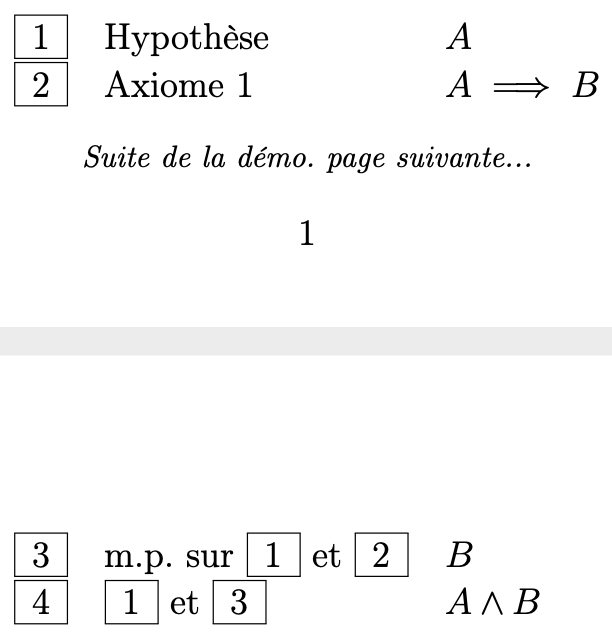
\includegraphics[scale = .5]{images/demo-explained-univ-broken[fr].png}}
\end{figure}

\end{document}
